\documentclass{article}

\usepackage{amsfonts}
\usepackage{amssymb}
%\usepackage{a4wide}
\usepackage{mathpartir}
\usepackage{amsthm}
\usepackage{indentfirst}
\usepackage{qtree}
\usepackage{graphicx}
\usepackage{listings}
\usepackage{color}

\definecolor{dkgreen}{rgb}{0,0.6,0}
\definecolor{gray}{rgb}{0.5,0.5,0.5}
\definecolor{mauve}{rgb}{0.58,0,0.82}

\lstset{frame=tb,
	language=Java,
	aboveskip=3mm,
	belowskip=3mm,
	showstringspaces=false,
	columns=flexible,
	basicstyle={\small\ttfamily},
	numbers=none,
	numberstyle=\tiny\color{gray},
	keywordstyle=\color{blue},
	commentstyle=\color{dkgreen},
	stringstyle=\color{mauve},
	breaklines=true,
	breakatwhitespace=true,
	tabsize=3
}


\begin{document}
		
	\title{
		Event Based Systems \\
		DEBS Grand Challenge 2019}
	\date{}
	\author{Balan Gheorghe
		\and Buruiana Sebastian
		\and Citea Alexandru
		\and Bute Iulian
	}
	
	\pagenumbering{arabic}
	
	\maketitle
	
	\tableofcontents{}
	
	\pagebreak
	
	\section{Data sets}
	
	We used the single-object data sets for training. For testing, we used the \texttt{set1} dataset provided, as it was the only dataset with multiple files. In order to have more data to test on, we made a generator which can create new data based on the data we have.
	
	The generator works like this. Say we want to generate a scene with $n$ objects. We randomly select $n$ objects (we also randomly select their projection) from the single-object dataset, we collect all points form all sensors and put them all together.
	
	The problem now is that there might be some sensors that generate more than 1100 points, which does not conform with the problem specification. In addition, the sensors might "see" objects which are behind other objects, even though that should not be possible in a real scenario (the light would be blocked by the object in front and it will not reach the object behind).
	
	In order to solve the later issue, we would like to find and eliminate all pairs of collinear points. However, due to precision errors, most points won't be exactly collinear. In order to address this issue, we compute the slope each points makes with the origin and choose the two points with the closest slopes (this is the pair of points which is closest to being collinear). From these two points, we remove the one that's further behind and then repeat the process until we have no extra points (i.e. we've reached the required 1100 readings).
	
	In addition to eliminating nearly collinear points, this method also has the upside of simulating a uniform rotation (since the maximal slope gap is minimized, which indirectly leads to all slope gaps converging to equal values). This behavior is desired if we want to simulate a real sensor.
	
	We've tested our program on sets generated by this method and we've obtained similar results to the ones on the provided data set, proving that the generator does indeed accurately simulate real world scenes.
	
	\section{The Parser}
	
	Our parser works in a semi-lazy way. We load the entire file content into memory, but regions of the file are only parsed and processed on demand, when needed. In the problem solution, different scenes are parsed individually by separate threads.
	
	We've plotted some of the objects we found in the data set. Below, we can see a projection of the \texttt{BmwX5Simple}, as it is given in the set (left). We can see that the object is encapsulated in a cylinder, which is not part of the object. We called this cylinder the \textit{environment}. In order to isolate the object, the Parser also has the role of removing the environment, in order to have all the data represent just the object itself. We can see what the same example looks like with the environment removed (right).
	
		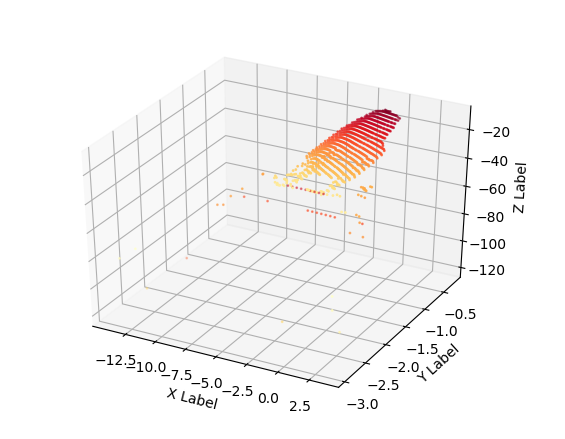
\includegraphics[width=0.9\textwidth]{img_nowall.png}
		
		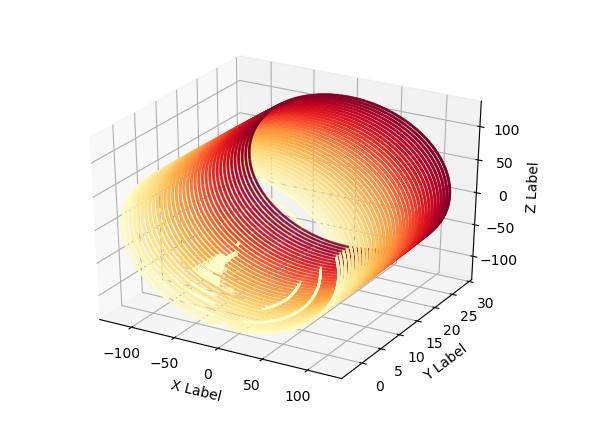
\includegraphics[width=0.9\textwidth]{img_wall.png}
	
	\section{Solution}
	
	\subsection{Training}
	
	For each object, we first eliminate noise via some heuristics (the environment was already eliminated by the parser). We then calculate its center of mass (by averaging out all points of the object) and then compute the mean squared difference from each of the points to this center. We repeat this for all projections of the object and average out all of these means, which results in a single number. This way, every object type is characterized by just one number.
	
	The advantage of this method is that this number condenses multiple bits of information: it is influenced by the object's shape, its size and various other factors.
	
	The disadvantage is that reducing an entire object to just one number might be somewhat superficial and it might lose some of the complexity of the objects. Also, somewhat similar to how hash collisions work, two different objects might end up having a similar characteristic number.

	\subsection{Testing}
	
	In order to test our solution on an instance with multiple objects, we first of all need to isolate said objects. For this, we use a standard implementation of the \texttt{DBSCAN} algorithm. We set the \texttt{min\_samples} parameter to 10 (the minimal number of points in a cluster), to help eliminate noise (in addition to the noise reduction heuristics we've mentioned before). We took all these precautions because we noticed that the data given is quite noisy. The \texttt{eps} parameter (arguably the most important one for this algorithm, the distance needed between two points in order to be considered neighbors) was chosen based on the scale of the coordinates in the input and was adjusted empirically thorough some runs.
	
	After the clusters are formed, we repeat the same process we used for training: we compute the center of mass and take the mean squared difference between all points and that center. This gives us the number. In order to categorize the cluster, we simply check which object has the closest characteristic number to this cluster's resulting number.
	
	\pagebreak
	
	\section{Benchmarks and results}
	
	Overall, the results are satisfying. We implemented the metrics as described by the formulas on the competition's web page, and on the \texttt{set1} test set, we've obtained the following results:
	
	\begin{center}
		\texttt{Accuracy: 0.42 Precision: 0.35 Recall: 0.57}
	\end{center}
	
	We've added benchmarks for various factors, as requested in the problem specifications. For the same test case mentioned above, on a laptop running an Intel Core i7, we've seen the following performance metrics:
	
	\begin{center}
		\texttt{Reading tuples / second: 0.1 | Solution latency: 0.44 | Solution throughput: 2.27}
	\end{center} 
	
\end{document}
